\chapter{Grundlagen}\label{ch:grundlagen}
In diesem Kapitel werden für diese Arbeit wichtige Begriffe und Systeme erläutert.

\section{Mainframe / Großrechner}\label{sec:mainframe}
Mainframe und Großrechner werden in dieser Arbeit gleichbedeutend verwendet.
Im modernen Sprachgebraucht kann ein Großrechner als größte zur Verfügung stehende Serverart betrachtet werden.
So wird er von Unternehmen verwendet, um dort kommerzielle Datenbanken, Transaktionsserver und Anwendungen, die einen hohen Grad an Sicherheit und Verfügbarkeit benötigten, zu hosten.
Im Gegensatz zu verteilten Serversystemen, bei dem die Funktionalitäten auf einzelne Server, wie zum Beispeil einen E-Mail-Server, einen Datenbank-Server, einen Web-Server usw. aufgeteilt sind, handelt es sich bei einem Mainframe um ein zentralisiertes System.
\cite{Ebbers.2011}

\subsection{Batch}
Batch beziehungsweise Batch-Verarbeitung ist eine Art einer Stapelverarbeitung.
Das heißt, dass Programme mit minimalem menschlichen Eingreifen nacheinander abgearbeitet werden.
Dies geschieht meist zu einer vorher festgelegten Zeit.
Zum Beispiel wird einmal am Tag zu einer ganz bestimmten Uhrzeit die Tägliche Bewertung der Rechnungsschreibung durchgeführt.
Die auszuführenden Programme sind in sogenannten Batch-Jobs definiert. 
\cite{Ebbers.2011}

\subsection{Batch-Job / Job}\label{ssec:job}
In einem Batch-Job, in dieser Arbeit wird Job gleichbedeutend verwendet, wird dem System mitgeteilt welches Programm mit welchen Eingaben und Ausgaben gestartet werden soll.
Dafür wird die `Job Control Language`, kurz JCL, genutzt.
Die drei Grundbausteine, die JCL breitstellt, werden im Folgendem beschrieben.

Zunächst ist `JOB` zu nennen, auch Jobkarte genannt.
Hier wird der Name des Jobs, Berechnungsinformationen, maximal zur Verfügung stehende CPU-Zeit und weitere Job weite Parameter gesetzt.

Innerhalb eines Jobs wird mit Hilfe des `EXEC` Befehls dem System mitgeteilt, welches Programm gestartet werden soll.
Es können mehrere `EXEC` Befehle in einem Job vorkommen, dabei wird jedes als einzelner sogenannter `Job step` bezeichnet.
Dabei können dem Programm neben den Eingabedateien auch weitere Parameter übergeben werden.

Als letztes ist der `DD` Baustein zu nennen.
`DD` steht für Data Definition.
Es verknüpft den Namen des Bausteins zum Beispiel an eine Datei, an ein I/O Gerät oder Funktionen, die im eigentlichen Programm enthalten sind.
So steuert es die Ein- und Ausgaben des Programmes.
Ein `DD` Baustein ist immer an ein `EXEC` Befehl gebunden.
Ein `EXEC` kann aber mehrere `DD` Bausteine enthalten.
\cite{Ebbers.2011}

\section{Customer Information Control System}\label{cics}
Das Customer Information Control System, kurz CICS, ist ein Applikationsserver für einen IBM-Großrechner.
Ein Applikationsserver stellt eine Umgebung zur Verfügung, in der Anwendungen gehostet werden können.
Dabei kümmert sich dieser unter anderem um Transaktionalität, Webkommunikation und Sicherheit.
Hierfür stellen Applikationsserver eine API zur Verfügung.
CICS hat einen weiteren Vorteil, es unterstützt verschiedene Programmiersprachen.
So können Programme innerhalb einer Anwendung in der für ihren Use-Case am besten geeigneten Sprache implementiert werden.
Zu den unterstützten Sprachen zählen neben COBOL und IBM Assembler auch Java und Java EE.
\cite{Rayns.2011}

\subsection{CICS Transaktion}\label{subsec:trans}
Ein Businessablauf wird im CICS in einer Transaktion gekapselt.
So kann eine Transaktion mehrere Programme unterschiedlicher Programmiersprachen umfassen.
Eine Transaktion besitzt ein eindeutiges Kürzel, die TransaktionsID.
Über die TransaktionsID kann der Ablauf gestartet werden.
Dies kann sowohl per Webanfrage oder per Messaging Queue als auch aus einem anderem Programm heraus oder per Hand geschehen.
In der Transaktion werden alle Änderungen die Programme an Resourcen, wie zum Beispiel einer Datenbank oder Dateien, tätigen protokolliert.
So wird im Fehlerfall sichergestellt, dass diese rückgängig gemacht werden können.
 \cite{Rayns.2011}

\subsection{Voraussetzungen}\label{subsec:voraus}
Im Umfeld der DATEV eG sind die Hard- und Softwarevorausetzungen um ein CICS beziehungsweise eine CICS Instanz zu erstellen und zu starten vorhanden.
Der Fokus dieser Arbeit liegt auf letzterem somit werden nur die dafür notwendigen Voraussetzungen dargelegt.
Außerdem liegt der Fokus nur auf Systemen, die vorerst nicht für die produktiven Systeme der DATEV eG vorgesehen sind.
Aus diesem Grund werden nur Schritte, die für ein solches Testsystem benötigt werden, dargestellt.
Eine weitere Eingrenzung besteht darin, dass nur die Arbeitsschritte, die mit z/OSMF\footnote{Beschreibung in Absatz \ref{sec:zosmf}} automatisiert werden, erläutert werden.

\subsection{Einrichtung CICS Instanz}\label{subsec:createCICS}
Die in diesem Absatz benötigten Informationen stammen aus Gesprächen mit Mitarbeiter 2 aus der Abteilung, die für die CICS Administration zuständig ist.
Um eine lauffähige CICS Instanz den Vorausetzungen aus dem Absatz \ref{subsec:voraus} entsprechend einzurichten, sind mehrere Schritte notwendig.
Diese werden im Folgendem beschrieben.

\subsubsection{CICS spezifische Dateien}\label{sssec:speziDat}
Zunächst müssen CICS spezifische Dateien im z/OS angelegt werden.
Im Falle dieser Arbeit handelt es sich um 17 verschiedene.
Diese Dateien benötigt die CICS Instanz um zum Beispiel Systemfehler zu protokollieren.
Eine weitere Datei ist dafür zuständig, dass ein Debugger innerhalb der Instanz verwendet werden kann.

\subsubsection{CSD}
In der CICS system defintion, kurz CSD, Datei muss jede Ressource, die dem System zur Verfügung stehen soll, definiert werden.
Eine CSD Datei kann für mehrere CICS Instanzen verwendet werden.
Eine solche allgemeine CSD Datei hat ca. 22.600 Einträge.
Ein Eintrag besteht aus einer Gruppe und einer Liste.
Die Gruppe ist hierbei die Definition einer Systemressource und muss händisch angelegt werden.
Bei der Liste handelt es sich um das System, welches diese Ressource benötigt.
Dort ist unter anderem für jede CICS Instanz hinterlegt, zu welchem Db2 Datenbanksystem und welchem MQ Messagingsystem sich diese Instanz verbinden soll.

\subsubsection{STC Job}
Bei einem Started Task Controll-Job, kurz STC Job, handelt es sich um einen Batch Job, der mit Hilfe des `START`-Konsolenkommandos innerhalb von z/OS gestartet werden kann.
Dieser Batch Job wird deshalb auch als Started Task bezeichnet.\cite{Cassier.2007}
Bei der DATEV eG existiert für jedes CICS ein solcher Job.
In diesem werden zunächst einige zur Laufzeit benötigten Bibliotheken und Dateien eingebunden, unter anderem die CICS spezifischen Dateien\footnote{Beschreibung in Absatz \ref{sssec:speziDat}}.
Außerdem werden hier die SIT \footnote{CICS system initialization table} Parameter definiert.
Zunächst wird festgelegt welche Standard SIT verwendet werden soll.
Anschließend können diese Standardwerte überschrieben werden.
Zu diesen Parameter zählen unter anderem, der eindeutige Name der CICS Instanz, der Speicherort der dazugehören CSD und ob eine Verbindung zu einem Db2 Datenbanksystem hergestellt werden soll.

\subsection{Entfernung CICS Instanz}
Um eine CICS Instanz zu entfernen muss diese zunächst gestoppt werden.
Dies ist über das `STOP`-Konsolenkommando von z/OS möglich.
Anschließend müssen alle im Absatz \ref{subsec:createCICS} beschriebene Schritte rückgängig gemacht werden.
Also müssen die für diese Instanz spezifischen Dateien, die Einträge für die CICS Instanz aus der CSD Datei und schließlich auch der STC Job gelöscht werden.

\section{IBM MQ}\label{sec:mq}
IBM MQ ist eine Messaging-Lösung der IBM.
Diese ermöglicht den asynchronen Datenaustausch zwischen Anwendungen mittels sogenannter Queues.
Alle IBM MQ Begrifflichkeiten, die in dieser Arbeit verwendet werden, werden im Folgenden erläutert.
\cite{Aranha.2013}

\subsection{Queue Manager}
Bei einem Queue Manager handelt es sich um die zentrale Ressource eines IBM MQ Systems.
So verwaltet er alle anderen IBM MQ Ressourcen.
Ausgenommen hiervon ist die Queue-sharing Group, diese ist für diese Arbeit aber nicht von relevanz.
Zur Verwaltung gehören unter anderem die Speichersteuerung der Daten und die Wiederherstellung dieser im Falle eines Fehlers.
Desweiteren koordiniert den Zugriff aller Anwendungen auf die Nachrichten in von ihm verwalteten Queues.
Um hierbei die Konsistenz sicherzustellen sorgt er für Locking und die notwendige Isolation.
\cite{Aranha.2013}

\subsection{Queues}
In Queues werden die Nachrichten, die von Programmen gesendet werden gespeichert.
Es gibt verschiedene Arten von Queues.

Die für diese Arbeit notwendigen sind zum einen die Local Queue.
Dabei handelt es sich um die einzige Queue Art, bei der die Nachrichten physikalisch gespeichert werden.
Alle anderen anderen müssen auf eine Local Queue zeigen.

Die andere ist eine spezielle Art von Local Queues, die sogenannten Initiation Queue.
Diese dient dem Queue Manager dazu unter bestimmten Bedingungen eine Trigger-Nachricht auf diese zu schreiben.
So kann eine andere Local Queue so definiert sein, dass sobald eine Nachricht auf sie geschrieben wird eine solche Trigger-Nachricht erzeugt werden.
Dies ermöglicht das Anwendungen nur starten, wenn wirklich Daten zum Verarbeiten vorhanden sind.
\cite{Aranha.2013}

\subsection{Process}
Für das Auslösen von Anwendungen wird nicht nur die Initiation Queue benötigt, sondern auch sogenannte Processes.
So muss der Local Queue, die eine Start einer Anwendung auslösen soll, bei der Definition nicht nur die Initiation Queue bekannt gemacht werden, sondern auch ein Process.
Ein Process legt den Type und den Namen der zu startenden Anwendung fest.
Als Type ist beispielhaft CICS oder auch WINDOWSNT für Windows unterstütze Platformen zu nennen.
Bei der Anwendung im Fall des CICS Types muss der Name der Transaktion angegeben werden.
Für Windows Platformen der Dateipfad der auszuführenden exe.
\cite{Aranha.2013}

\section{IBM Cloud Provisioning and Management for z/OS}\label{sec:zosmf}
In diesem Absatz wird zunächst auf die für dieses Kapitel grundlegenden Begriffe eingegangen.
Anschließend wird IBM Cloud Provisioning and Management for z/OS, kurz z/OSMF, erläutert.
Im Anschluss darauf wird das auf Kommandozeilenbefehle basierende z/OS Provisioning Toolkit, kurz z/OS PT, und dessen Möglichkeiten dargestellt.

\subsection{Begrifferklärung}
Im folgenden werden einige allgemeine Begriffe, die im Umfeld von IBM Cloud Provisioning and Management for z/OS vorkommen, erläutert.

\subsubsection{Provisioning}
Ins Deutsche übersetzt bedeutet es Bereitstellung, in dieser Arbeit wird auch Provisionierung verwendet.
In dieser Arbeit umfasst dieser Begriff die Bereitstellung einer Laufzeitumgebung beziehungsweise den Prozess, der hierfür benötigt wird.

\subsubsection{Workflow}\label{sssec:workflow}
Ein Workflow ist eine beliebig komplexe eindeutige Aneinanderreihung von sogenannten Steps.
Nach der Ausführung dieser wird ein bestimmtes Ziel erreicht, zum Beispiel die erfolgreiche Bereitstellung eines CICS Systems.
Die Definition eines Workflows, den dazugehörigen Steps und ihrer Variablen wird in XML umgesetzt.
Ein Step beschreibt einen Teilablauf eines Workflows.
Innerhalb eines Steps können sowohl interne und externe Scripte als auch JCLs und somit Programme ausgeführt werden.
Des weiteren besteht die Möglichkeit REST-Calls zu tätigen.
Außerdem können Bedingungen für die Durchführung eines Steps definiert werden.
So ist es zum Beispiel möglich einen Step nur durchzuführen, wenn eine bestimmte Variable einen bestimmten Wert besitzt.
Ein weiteres Beispiel ist, es können erforderliche Steps definiert werden, so dass bevor ein Step auf eine Datei zugreift, mittels eines vorherigen Steps geprüft wird ob diese vorhanden ist und wenn nicht diese erzeugt.
Es wird ein XML Schema verwendet um sicherzustellen, dass zur Laufzeit keine syntaktischen Fehler vorhanden sind.
\cite{Rotthove.2018}

Ein Nachteil von Workflows ist, dass diese statisch sind, das heißt, dass die Variablenzuweißungen immer zum Zeitpunkt der Erstellung stattfindet.
Dadurch ergibt sich, dass für jede kleine Änderung ein eigener Workflow erzeugt werden muss.
Somit ist ein Workflow eher ein Einmal- bzw. Wegwerfprodukt.

\subsubsection{Template}
Bei dem Nachteil von Workflows als Wegwerfprodukt setzen die sogenannten Templates an.
Ein Template besteht aus drei Dateien.

Einer Datei für Eingabevariablen.
In dieser Datei können Workflowvariablen Werte zugewiesen werden.
Diese Variablen müssen bei ihrer Definition im Workflow entsprechend gekennzeichnet sein.

Die nächste Datei ist die sogenannte Aktion-Definitions-Datei.
Hier werden die Aktionen, die ein Anwender mit diesem Template durchführen kann, festgelegt.
Einer Aktion wird eine Workflow Definitions Datei und somit ein Workflow zugewiesen.
Dabei ist zu beachten, dass die Datei für die Eingabevariablen und welche Variablen davon verwendet werden, anzugeben ist.

Als letzte Datei ist die Manifest-Datei zu nennen.
In dieser wird dem Template mitgeteilt an welchem Speicherort sich die oben genannten Dateien befinden.
Da ein Template immer provisioniert werden kann, wird hier auch der Speicherort des Bereitstellungsworkflows angeben.
Zusätzlich kann noch eine Beschreibung des Templates hinzugefügt werden.

Somit bildet ein Template einen Rahmen um mehrere Workflows und ermöglich so schnellere De-/provisionierung.
Zudem können die Variablen nur an einer Stelle geändert werden.
Außerdem besteht die Möglichkeit, den Variablen zum Zeitpunkt der Provisionierung als Anwendereingabe einen Wert zuzuweisen.
Somit ist ein Template flexibler als ein Workflow.
\cite{IBM.2019}

\subsubsection{Instance}
Hierbei handelt es ich um das Ergebnis nach der Provisionierung eines Templates.
Zum Beispiel eines funktionsfähigen CICS.

\subsection{IBM Cloud Provisioning and Management for z/OS}
Das IBM Cloud Provisioning and Management for z/OS bietet die Möglichkeit mehrere Systeme innerhalb eines z/OS Betriebssystems zu provisionieren, unter anderem Laufzeitumgebungen wie CICS.
Jedoch nicht die Bereitstellung eines kompletten z/OS Betriebssystems.
Für diese Aufgaben stehen zwei Schnittstellen zur Verfügung.
Zum einem z/OS Provisioning Toolkit, im Weiteren z/OSPT genannt, und zum anderen z/OS Management Facility, im Weiteren z/OSMF genannt.
\cite{KeithWinnardGaryPuchkoffHirenShah.2016}

\subsubsection{z/OS Provisioning Toolkit}\label{sssec:zospt}
z/OSPT bietet ein Kommandozeileninterface für die Bereitstellung und das Verwalten von Laufzeitumgebungen.
In Abbildung \ref{fig:zospt_help} werden die möglichen Kommandozeilenbefehle mittels des Befehls `zospt -h` in einem Kommandofenster angezeigt.
\begin{figure}[h]
	\centering
	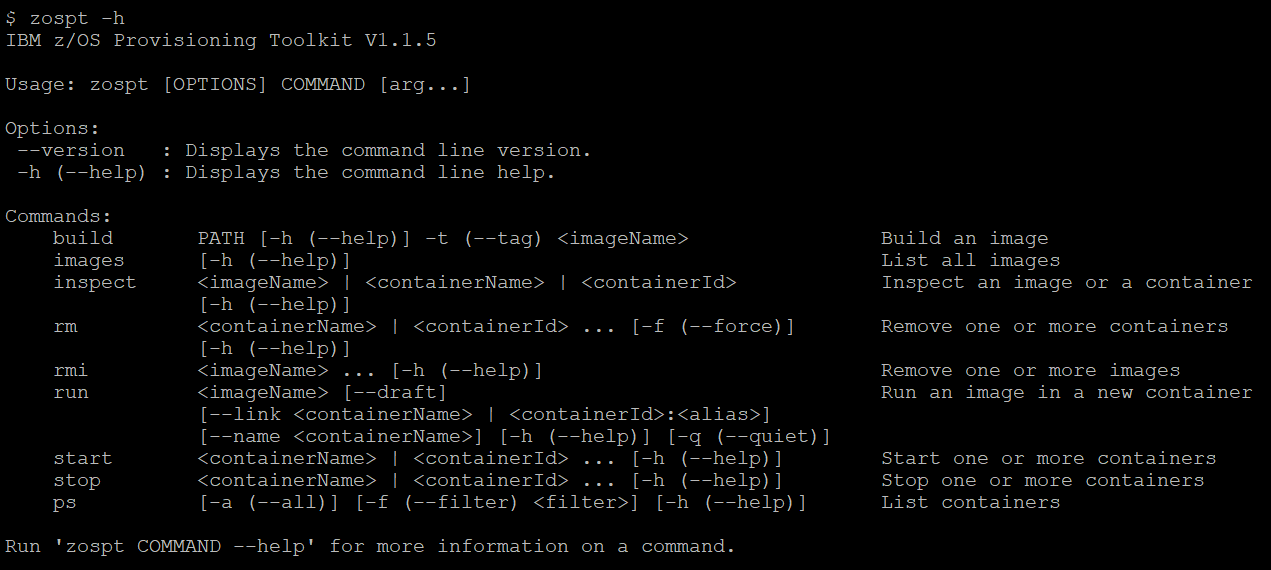
\includegraphics[width=\textwidth]{figures/zospt_help_putty.png}
	\caption{z/OSPT mögliche Kommandozeilenbefehle}
	\label{fig:zospt_help}
\end{figure}
Mit z/OSPT werden noch zwei weitere Begriffe eingeführt.\\
Zum einen sogenannte `images`.
Dabei handelt es sich grundsätzlich um ein Template, jedoch kann dieses Template über eine weitere Inputfile verändert werden.
Dadurch kann ein Template mit kleineren Änderungen provisioniert werden, ohne dass ein neues Template erzeugt werden muss.
Dies erhöht die Flexibilität weiter.\\
Des anderen die sogenannten `container`.
Dabei handelt es sich eins zu eins um eine Instance.
\cite{IBM.2019b}

\subsubsection{z/OS Management Facility}\label{sssec:zosmf}
Der Hauptaugenmerk dieser Arbeit liegt jedoch bei z/OSMF.
Da dieses die Verwaltung von Workflows und Templates über eine browserbasierende Schnittstelle ermöglicht.
Durch diese Oberfläche, in Abbildung \ref{fig:zosmf_welcome} dargestellt, ist es einfacher zu bedienen und somit wird der Einstieg in die Provisionierung erleichtert.

//hier zosmf welcomepage screenshot

Wie auf der rechten Seite der Abbildung \ref{fig:zosmf_welcome} zu sehen ist, bietet z/OSMF viele Funktionen an.
Für diese Arbeit besitzt nur der Menüpunkt `Cloud Provisioning` Relevanz.
Unter diesem Punkt sind die Funktionalitäten für die automatisierte Bereitstellung von Templates zu finden.
\cite{Rotthove.2018}

Dabei handelt es sich zunächst um das `Resource Management`.
Darunter werden sogenannte `Domains` und die dazugehörigen `Tenants` verwaltet.
Unter einer `Domain` ist ein System, das Systemressourcen in Ressourcenpools gliedert, zu verstehen.
`Tenants` sind die dazugehörigen Rechtegruppen, die dem Anwender den Zugriff und die Nutzung von zugeordneten Templates ermöglicht.
Einem Template muss sowohl eine `Domain` als auch ein `Tenant` zugewiesen werden.
\cite{Rotthove.2018}

Zur Verwaltung der Templates und Instances kommen die `Software Services` zum Einsatz.
Dort können neue Templates über Manifest Datei hinzugefügt werden.
Dann muss, wie oben beschrieben, eine `Domain` und ein `Tenant` zugwiesen werden.
Anschließend kann das Template, falls es keine Fehler beinhaltet, veröffentlicht werden.
Es ist zu empfehlen vorher einen `Test Run` durchzuführen.
Dabei wird eine Instance testweise provisioniert.
Diese Instance verhält sich genauso wie eine Instance, die aus einem veröffentlichten Template erzeugt wurde.
Somit kann damit das Template und die in der Aktion-Definitions-Datei definierten Aktionen getestet werden.
\cite{Rotthove.2018}
